\documentclass[a4paper,11pt]{article}
\usepackage[utf8]{inputenc}
\usepackage{lastpage}
\usepackage{fancyhdr}
\usepackage[english]{babel}
\usepackage[a4paper,margin=1in]{geometry}
\usepackage{multirow}
\usepackage[table,xcdraw]{xcolor}
\usepackage{array}
\usepackage{graphicx}
\usepackage{caption}
\usepackage{ctable}
\usepackage{listings}

\newcolumntype{L}[1]{>{\raggedright\let\newline\\\arraybackslash\hspace{0pt}}m{#1}}
\newcolumntype{C}[1]{>{\centering\let\newline\\\arraybackslash\hspace{0pt}}m{#1}}
\newcolumntype{R}[1]{>{\raggedleft\let\newline\\\arraybackslash\hspace{0pt}}m{#1}}

\newcommand\tab[1][4mm]{\hspace*{#1}}


%-------------------------------------------------------------------------------
% HEADER & FOOTER
%-------------------------------------------------------------------------------

\pagestyle{fancy}
\fancyhf{}
\setlength\headheight{15pt}
\fancyhead[L]{ Imaging Lab 2 }
\fancyhead[R]{Student ID: 100633486}
\fancyfoot[R]{Page \thepage\ of \pageref{LastPage}}


%-------------------------------------------------------------------------------
% TITLE PAGE
%-------------------------------------------------------------------------------

\begin{document}

\title{
	\Huge \textbf {Color and Contrast}
    \\ [0.2cm]
	\LARGE Imaging Lab 2 - May, 2017
    \\ [0.5cm]
    \hrule
}

\date{}

\author{
		\Large Kamyar Nazeri \\
		\large Student ID: 100633486 }

\maketitle
\newpage

\section*{Cancer cells detection mask}
To produce a detection mask, we apply RGB color thresholding on the reference image. To find the color thresholds, we need to know the location and color of the cancer cells. We can extract the cancer cells from the reference image by multiplying it with the provided ``true mask". We can then use the ``thresh" GUI tool to find the color threshold required for the detection mask. The color thresholds are at their best, when changing the Original Image from ``tissue" to ``cancer only cells" would not change the produced Mask. \\
\emph{Figure 1} shows the reference image, along side the extracted cancer cells, and normal cells:

\begin{figure}[!htb]
  \centering
  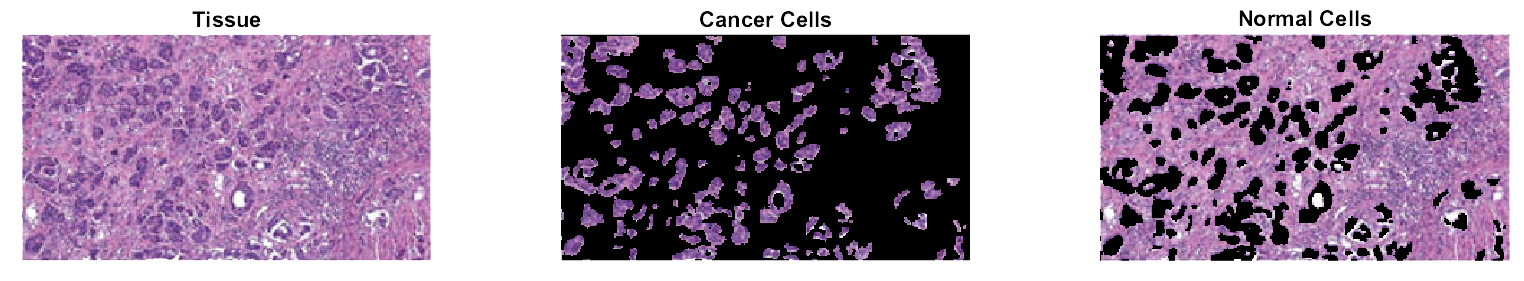
\includegraphics[width=16cm, height=4cm]{1.png}
  \caption{\small Extract cancer/normal cells from the reference image using the provided mask}
\end{figure}

 \\\\
To enhance the quality of the detection mask, we apply ``binary image operations" on the detection mask. We use \textbf{\emph{Dilation}} to grow the blobs, \textbf{\emph{Fill}}, to fill the black regions surrounded by white pixels and \textbf{\emph{Area Open}}, to remove all blobs having small areas. The followings are the color thresholds and binary operations we use to produce the detection mask: \\\\
\tab Red: 0 - 129 \\
\tab Green: 0 - 79 \\
\tab Blue: 116 - 255 \\
\tab Dilation: A disk with radius of 2 \\
\tab Area Open: Remove all blobs that have an area smaller than 50 \\
\tab Fill:  Fill in black regions that are completely surrounded by white pixels \\

 \\
\emph{Figure 2} shows the detection mask produced by color thresholding, alongside the mask after performing binary image operations:

\begin{figure}[!htb]
  \centering
  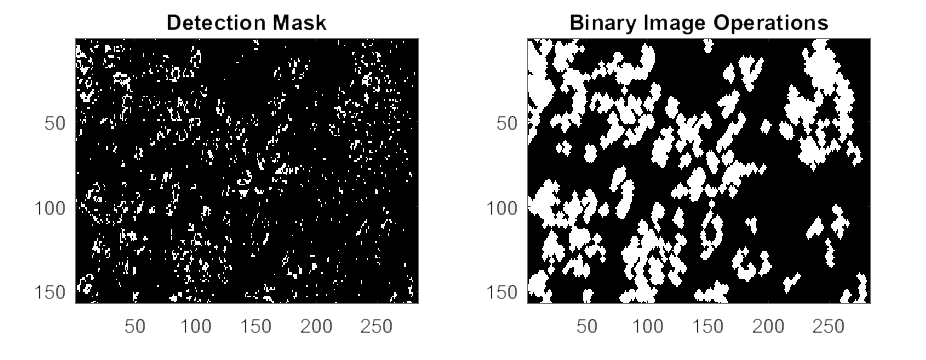
\includegraphics[width=14cm, height=5cm]{2.png}
  \caption{\small The detection mask produced by color thresholding / performing binary image operations}
\end{figure}

\newpage
 \\To measure the quality of our binary detection mask, we use \emph{Matthews correlation coefficient} (MCC) and compare our detection mask with one provided. In our simulation, we reached the value of \textbf{0.6063}. \\
The following table displays the 5 statistics used to evaluate the detection result:

\begin{center}
\setlength\extrarowheight{6pt}\large
\begin{tabular}{|C{3.5cm}|C{1.5cm}|C{1.5cm}|C{1.5cm}|C{1.5cm}|C{1.5cm}|}
\cline{2-6}
\multicolumn{1}{c|}{} & \textbf{TP} & \textbf{TN} & \textbf{FP} & \textbf{FN} & \textbf{MCC} \\ \hline
Detection Mask & 2319 & 33035 & 576 & 8658 & 0.3394 \\ \hline
Binary Image Operation & 8461 & 29161 & 4450 & 2516 & 0.6063 \\ \hline
\end{tabular}
\end{center}

\par\noindent
\emph{Classification categories, from left to right: True Positive (TP), True Negative (TN), False Positive (FP), False Negative (FN) and the Matthews Correlation Coefficient (MCC)}

 \\
\emph{Figure 3} qualitatively compares our detection mask to the provided mask by displaying the detection mask next to ``true mask":
\begin{figure}[!htb]
  \centering
  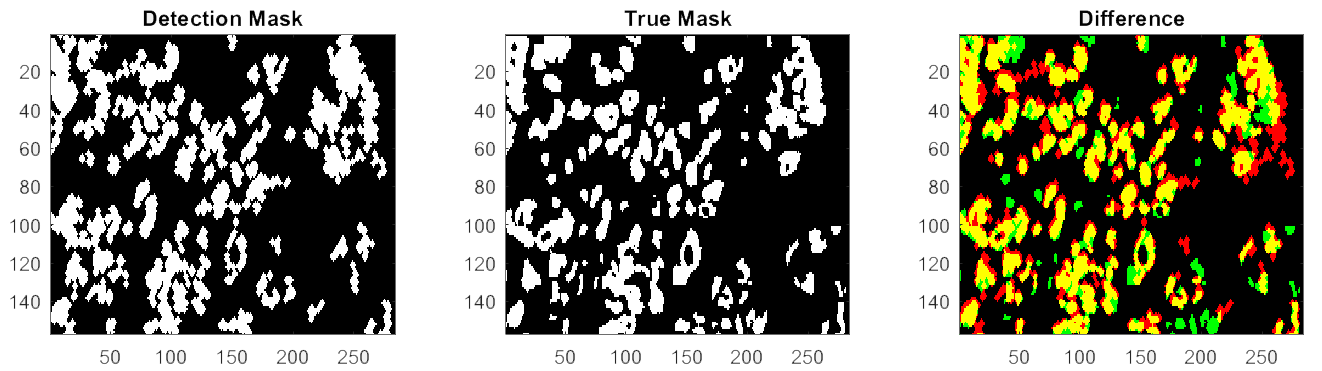
\includegraphics[width=16cm, height=4cm]{3.png}
  \caption{\small Visualization of the difference between the detection mask and the ``true mask"}
\end{figure}

\section*{Histogram equalization / HSV thresholding.}

We can improve our detection mask using, histogram equalization (Lab2\_3.m) and HSV thresholding (Lab2\_2.m). The following table demonstrates the statistics for RGB thresholding and the improved versions:
\begin{center}
\setlength\extrarowheight{6pt}\large
\begin{tabular}{|C{4.5cm}|C{1.5cm}|C{1.5cm}|C{1.5cm}|C{1.5cm}|C{1.5cm}|}
\cline{2-6}
\multicolumn{1}{c|}{} & \textbf{TP} & \textbf{TN} & \textbf{FP} & \textbf{FN} & \textbf{MCC} \\ \hline
RGB thresholding & 2319 & 33035 & 576 & 8658 & 0.3394 \\ \hline
HSV thresholding & 7543 & 25547 & 8064 & 3434 & 0.4039 \\ \hline
Histogram equalization & 7543 & 25547 & 8064 & 3434 & 0.4193 \\ \hline
\end{tabular}
\end{center}


\newpage

\end{document}
